\documentclass[11pt]{article}   
\usepackage{fullpage}      
\usepackage{color}
\usepackage{hyperref}
\usepackage{cite}
\usepackage{graphicx}
\usepackage{placeins}
\graphicspath{{./images/}}

\hypersetup{
    colorlinks,
    citecolor=black,
    filecolor=black,
    linkcolor=blue,
    urlcolor=blue
}

\begin{document}

\title{\bf CPSC 526 - Final Report \\ \emph{Public Key Web Authentication}}
\author{Masud Khan, Kyle Milz, Jeff Nicholson}
\date{April 16, 2012} 
\maketitle

\tableofcontents
\pagebreak
\begin{abstract}
Passwords are a necessary part of everyones online activities. They are also a pain. Remembering strong, unique passwords for multiple sites is extremely difficult. This results in users relying on weak passwords, like '123456', which leads to security and privacy concerns. What if there was a way to handle authentication that did not rely on passwords? We hope to provide such an authentication system. We suggest using public key cryptography, which after initial set up, allows users to seamlessly and securely authenticate to web sites, without the need for cumbersome passwords.\\
We will provide a simple authentication protocol, lightweight server side implementation and browser plug in, which can be easily adopted by anyone. A lightweight server side implementation means service providers do not need to make large changes to their implementations. A browser plug-in handles the client side and hides the authentication process from the user, allowing seamless, secure authentication.
\end{abstract}
\pagebreak


\section{Introduction} \label{sec:intro}
Authentication is an important part of our online activities. If you have an account with a web service, in order to log in you must authenticate yourself to the server. This ensures that you are the owner of the account. Almost all web sites currently use the username/password paradigm for authentication. Upon signing up for an account, the user provides a username or email, and a password. These are stored by the service, hopefully properly hashing the password, so that when the user returns, they provide their username and password, and the server can verify the information matches that in its database. This method works in theory, but there are problems (Seciton \ref{sec:webauth}). Weak passwords, managing many passwords, forgetting passwords are some examples, more are discussed in Section \ref{subsec:passwords}.\\
Current solutions exist to help users to create and manage more secure passwords. These include \nameref{subsec:pwdhash}, 1Password, and KeePass. Most modern browsers allow you to save passwords for websites you visit, these are often stored in plain text. While these solutions are helpful, they don't solve the inherent problem. Web Authentication can be handled without the username/password paradigm all together. By utilizing well known methods of Public Key Authentication, and tying current key management tools to the browser, we can create a secure, easy to use, web authentication system.\\
The goal of our project is to create and implement a Public Key Web Authentication system. This paper describes the protocol we used (Section \ref{sec:protocol}), the implementation details of our system (Section \ref{sec:implementation}), as well as applications (Section \ref{sec:applications}) and improvements to the system (Section \ref{sec:limitations},\ref{sec:futureWork}). The code for this project is available on GitHub \cite{526proj}. 


\section{Web Authentication} \label{sec:webauth}
When a user wants to log into their account on a web service, the server hosting the service must verify that the user is the valid owner of the account. This is the purpose of authentication. Authentication is also useful in the other direction. The user should be able to verify they are communicating with a server they can trust.\\
Authentication on the web is available through protocols such as SSH, TLS and HTTPS, which provide mutual authentication and secure communication between parties. These, however, do not provide authentication at the application layer, in the form of authenticating a specific user to their personal account on a server. Something similar, using symmetric or asymmetric keys, but at the application layer would be ideal for web authentication. This is exactly what public key web authentication does.  
\subsection{Passwords} \label{subsec:passwords}
The current standard for web authentication is password verification. The user provides a chosen password to the server, which verifies the password is correct, then provides the client access. There are multiple problems with this system.\\
You are trusting that the server is going to protect your password. This means properly storing it, as a hashed and salted value, not in plain text. If the server is compromised you do not want your password exposed. This risk can also be mitigated by using different passwords for every account. This means users must remember many unique non-trivial passwords. This is not simple, and many users choose not to do this. Users consistently re-use passwords for multiple accounts \cite{domino}. Even users who choose to use different passwords, often choose very naive, simple passwords, which are easy for an adversary to break \cite{habits}. It would be far simpler and more secure if users just had to remember one simple passphrase, which would control access to every account they had. This is what public key web authentication provides. 
\section{Protocol} \label{sec:protocol}

\subsection{Overview} \label{subsec:overview}
The public key web authentication protocol we implemented is based on classic challenge response. The client and server both have a public private key pair. In order for the client to verify the server identity, they encrypt a random nonce with the expected servers public key. This is sent to the server, which then must decrypt the nonce and send it back in plain text to the client. If what the client receives is the same as the nonce it encrypted, it knows that it is communicating with who it thinks. The process is symmetric for the client to authenticate itself to the server. Upon signing up for a new account, the client provides an email address, which the server uses to look up the clients public key from the key repository. When the client visits the site, its public key ID is provided automatically. The server encrypts a random nonce with the clients public key, and sends it to the client. The client must then decrypt and reply back to the server. The server verifies that the response matches. If so, it can be sure that the client has the private key corresponding to the public key for the client owning the account, thus authenticating the client.\\
The protocol consists of optional server authentication, then three stages in which the client is authenticated. Protocol messages are passed through HTTP headers. Keys are managed by external software on the client and server machine. Our implementation uses GnuPG, see Section \ref{sec:implementation} for more details. We also utilize a distributed public key repository to look up public keys.\\
Once authenticated the user is granted a secure session cookie, which allows them to access secure content.

\subsection{Server Authentication} \label{subsec:serverAuth}
optional server auth description
\subsection{Stage 0} \label{subsec:stage0}

\subsection{Stage 1} \label{subsec:stage1}

\subsection{Stage 2} \label{subsec:stage2}

\subsection{Session Management} \label{sessionManagement}
Describe cookies, how prevent session hijacking.


\section{Implementation} \label{sec:implementation}
The implementation consists of both a client side and server side. They are simple and not robust, more just a proof of concept showing the protocol described in Section \ref{sec:protocol} could be implemented. The implementation is an extension of existing work by Kyle Huff, gpgAuth \cite{gpgauth}. gpgAuth provided us with a browser extension, which we modified slightly, and a skeleton server implementation in PHP. We added features to this implementation to make it easier to use and integrate into existing systems. We also ported it to three other languages commonly used in web back ends; Perl, Python, and Ruby. Our hope is to allow sites to adopt this system without having to worry that the language they use is not supported. 

\subsection{Client Side}
The client side implementation uses existing key management software GnuPG to manage keys. The browser extension interacts with this through an API written in CPP, namely gpgauth-npapi \cite{npapi}. The open source extension is for Chrome/Chomium browser and was originally written by Kyle Huff \cite{ext}. We forked his project \cite{extFork}, and made some slight modifications to encoding to suite our needs.  
\subsubsection{Goals}
The client side needs to be simple to use. After initial set up, we want the user to be able to seamlessly authenticate with sites. We want minimal keyboard input or other interaction from the user. The work should be carried out transparently behind the scenes, then provide the user with visual confirmation of authentication.

\subsubsection{GPG}
Gnu Privacy Guard (GPG) is a free implementation of the OpenPGP standard as defined by RFC4880 \cite{gpg}. It allows users to manage public/private key pairs, and encrypt, decrypt and sign data. It provides a command line interface that can interact with applications through various libraries. GPG is used in our implementation to manage the client and server key rings. It is used to encrypt and decrypt the random nonces used for authentication.\\
With GPG users can easily create a key pair, and protect their private key with a strong passphrase. They are then able to publish their public keys to a public key server. Our implementation uses SKS OpenPGP Keyservers \cite{sks}, specifically the Ubuntu key server \cite{ubuntuKey}, although SKS keeps the entire pool of key servers synchronized.\\
GPG also provides users with the ability to revoke public keys. This is important if a user's private key is compromised. They are able to revoke their public key on the key servers. Then when someone tries to authenticate using the compromised key, the web service server will look up the key from the key server and realize it has been revoked.\\
The ability of users to sign other users public keys is crucial to the success of any public key authentication scheme. A web of trust between users gives them an idea how much a particular public key or signature should be trusted \cite{weboftrust}.\\
Our implementation needs users to generate a key pair with GPG, and publish their public key to the SKS OpenPGP Keyservers. Once this is done, they can set up the browser extension, which interfaces with GPG, and all authentication will be handled seamlessly. The user only has to occasionally enter their private key passphrase.

\subsubsection{Browser Extension}
The browser extension is build specifically for the Chrome/Chromium browser. It is written in Javascript. It was created by Kyle Huff as part of the gpgAuth project. We modified it slightly to suit our needs. Throughout work on this project we found many areas where the extension could be improved, but due to time constraints did not pursue them. See Section \ref{sec:futureWork} for more details.\\
The extension has multiple dependencies. In order for it to function, these need to be properly installed on your system. The extension setup checks your system to ensure these are working, see Figure \ref{fig:ext_setup_check}.\\
\begin{figure}[h!]
\centering
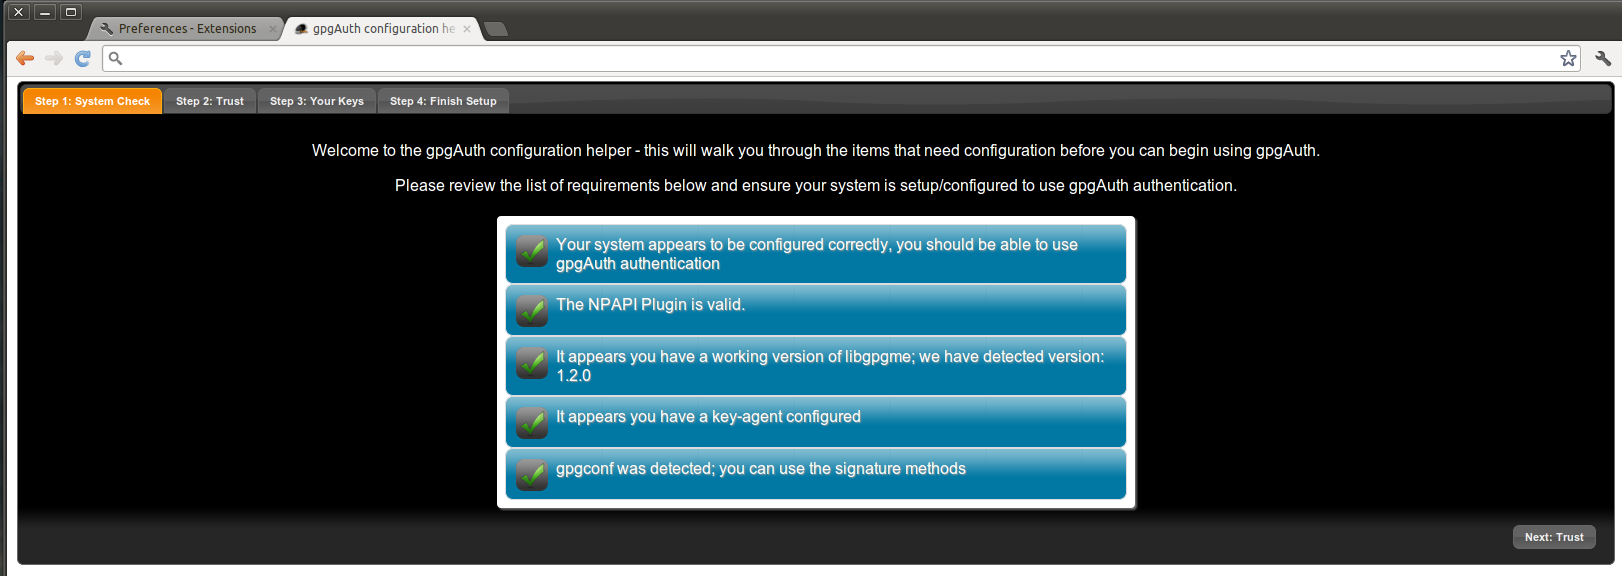
\includegraphics[scale=0.3]{ext_setup_systemCheck}
\caption{Screen shot of extension system check during setup}
\label{fig:ext_setup_check}
\end{figure}

The extension requires the npapi plugin, which is the interface between the extension and GPG. See Section \ref{subsubsec:npapi} for more details. The plugin requires libgpgme, which is an API that allows applications to easier interact with GPG. Key-agent is a program that handles the users passphrase for private keys. It is separate from the extension, so that when the user has to enter their passphrase it occurs locally and has no interaction with the insecure browser. Gpgconf allows applications to automatically modify GPG files. This allows for key signing and modification of a users key ring on the fly by an application. This way during setup you can sign keys from the extension. Also you can sign servers public keys during authentication.\\
After a successful system check, the extension prompts you to choose select your minimum trust level. Level 0 is the most stringent, and requires that domains you authenticate to have public keys which are signed by one of your ultimately trusted keys. The least stringent level, Level 8, only requires that the servers public key be signed by a key you trust. These levels of trust can be seen in Figure \ref{fig:trust}. They change the type of prompts you will see when authenticating to a server, but you can always choose to proceed with authentication even if the server does not meet your trust requirements, Figure \ref{fig:untrusted} shows the prompt you see in this case, you can choose log in anyway.\\

\begin{figure}[h!]
\centering
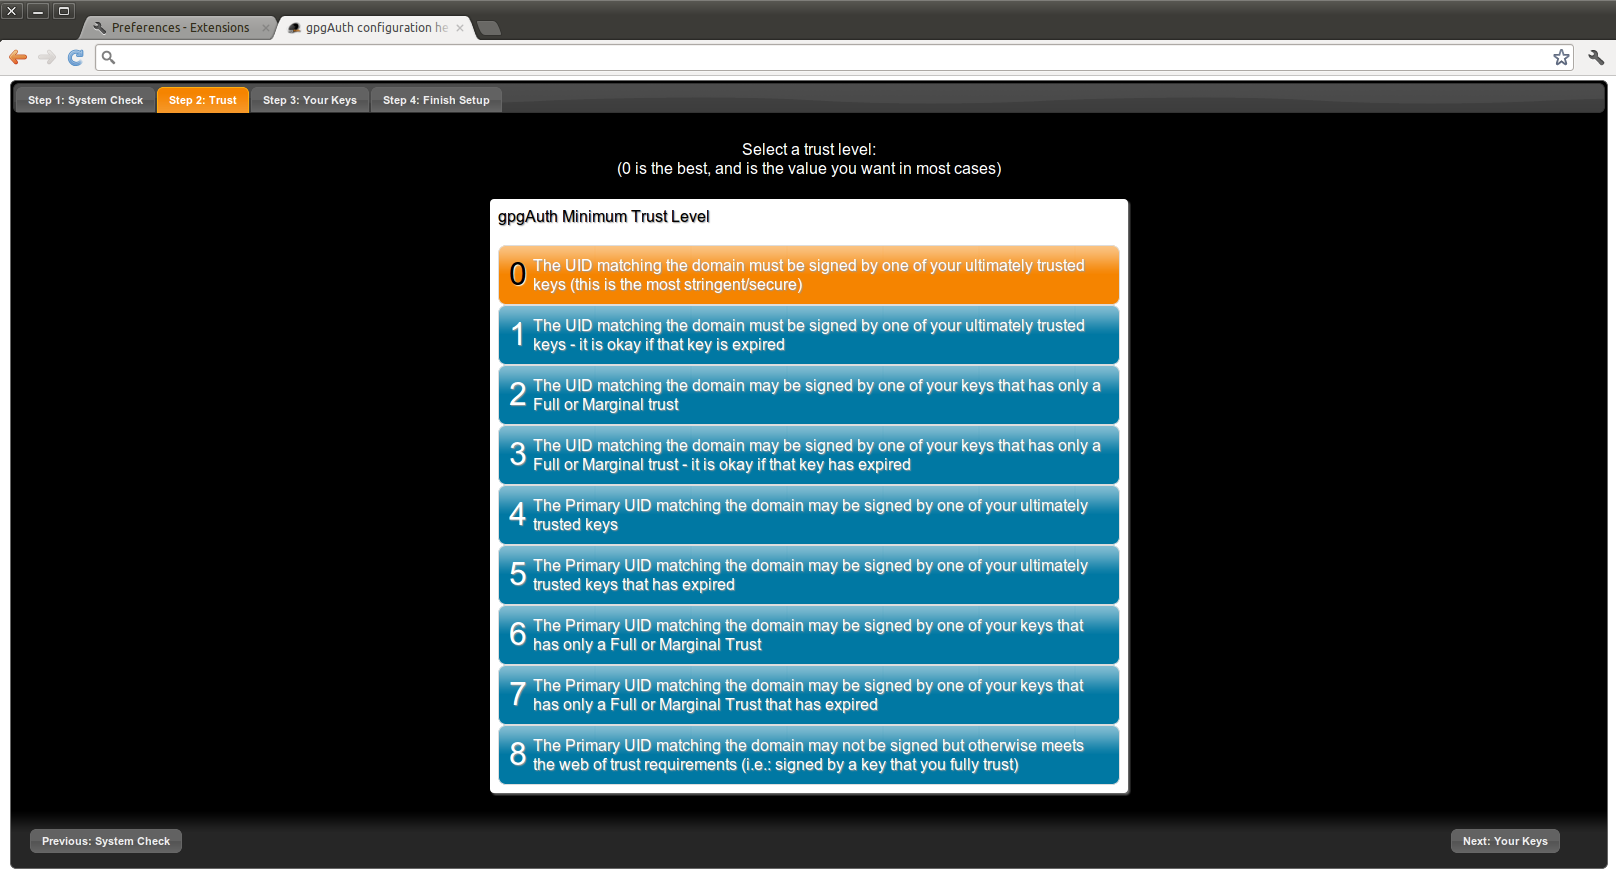
\includegraphics[scale=0.3]{ext_setup_trust}
\caption{Screen shot of extension trust levels}
\label{fig:trust}
\end{figure}

\begin{figure}[h!]
\centering
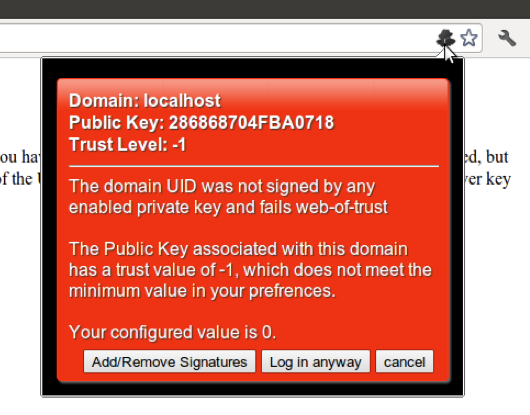
\includegraphics[scale=0.5]{ext_loginNotSigned}
\caption{Prompt shown by extension when the key of the domain does not meet your minimum trust requirements}
\label{fig:untrusted}
\end{figure}

The next step of setup ensures that you have a key pair generated. Figure \ref{fig:keysetup} shows this step. It will allow you to generate a new key through the extension.\\
\begin{figure}[h!]
\centering
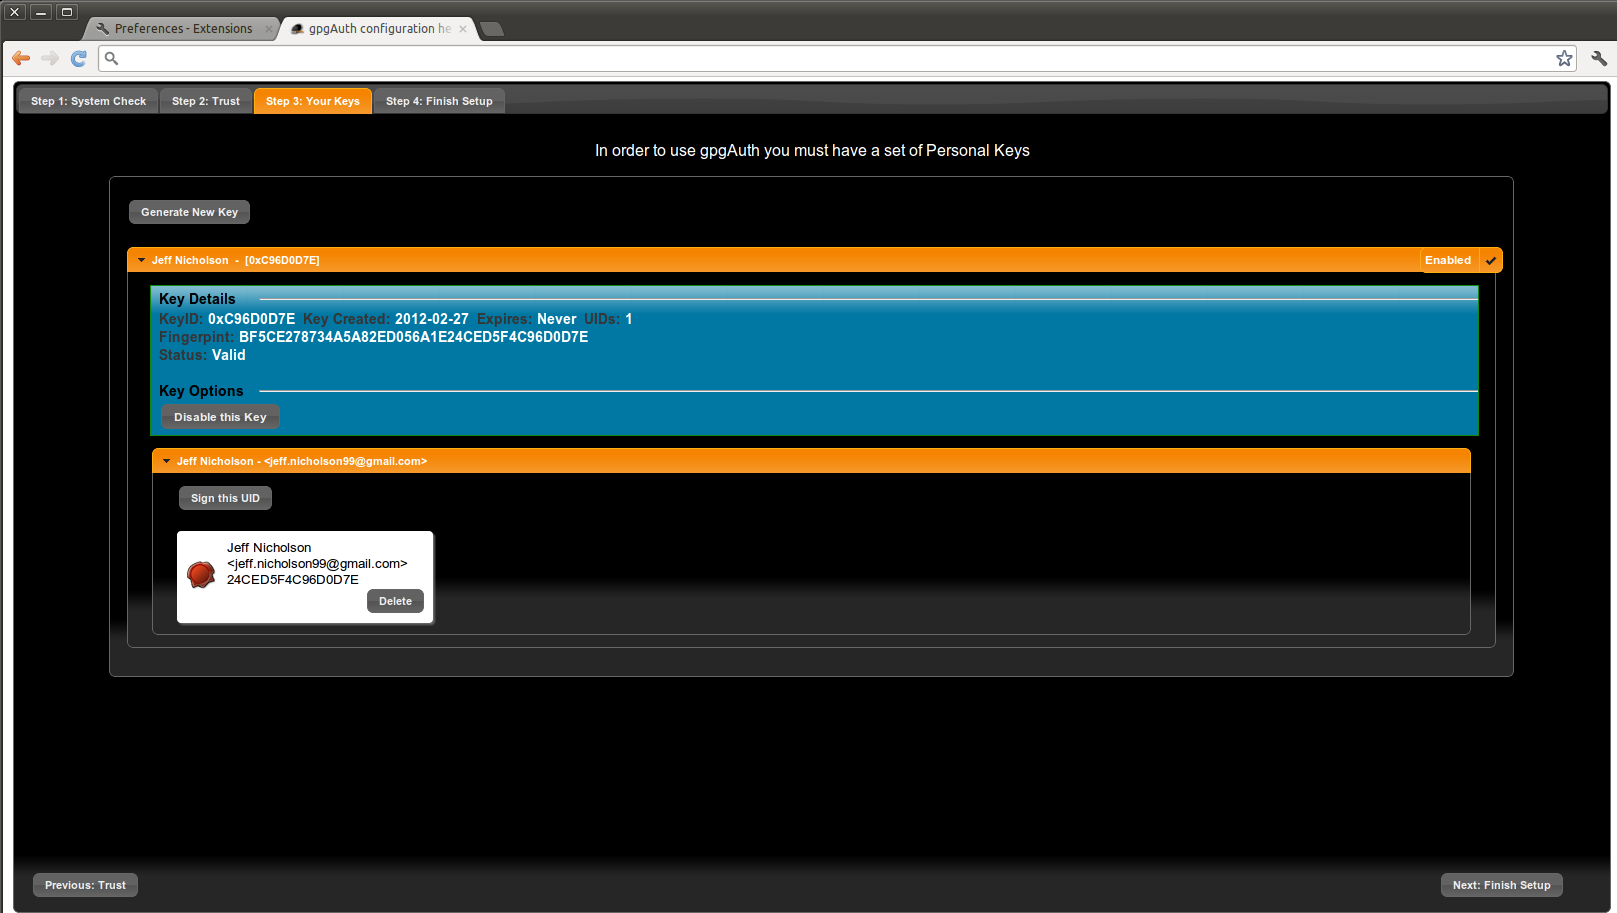
\includegraphics[scale=0.3]{ext_setup_keys}
\caption{Extension key setup}
\label{fig:keysetup}
\end{figure}

Once setup is complete, you can begin using the extension to authenticate to domains that implement the protocol. When you visit a domain with the protocol implemented, an icon will show up next to the browsers address bar. By clicking the icon you will be able to login, or logout if already logged in. Figure \ref{fig:login} shows the prompt when clicking on the icon to login. Figure \ref{fig:logout} shows the prompt to logout. This figure also shows the icon with the addition of a lock. The lock appears when you have successfully authenticated to the domain.\\
\begin{figure}[h!]
\centering
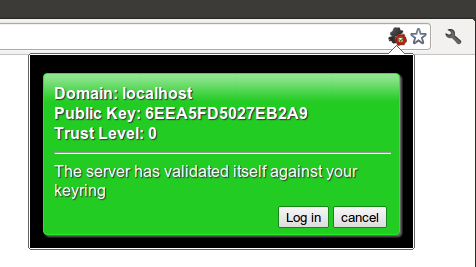
\includegraphics[scale=0.5]{ext_login}
\caption{Logging in. The icon only appears for sites that implement the protocol}
\label{fig:login}
\end{figure}

\begin{figure}[h!]
\centering
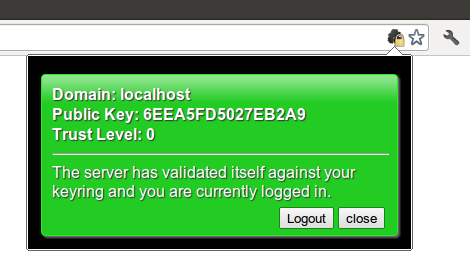
\includegraphics[scale=0.5]{ext_logout}
\caption{Logging out. Note the lock over the icon, this means you are currently authenticated}
\label{fig:logout}
\end{figure}

\FloatBarrier
\subsubsection{gpgauth-npapi} \label{subsubsec:npapi}

\subsection{Server Side}
The server side implementation is based on work done by Kyle Huff \cite{gpgauth}. We took his open source PHP back end, and modified it making it easier to use. We then ported it to other languages to make it easier to adopt.
\subsubsection{Goals}
The main goal with the server implementation is to make it easy to adopt. Sites currently using the standard method of password authentication are not going to want to make large infrastructure changes in order to adopt a new method of authentication. By creating single modules that handle the authentication process as described in Section \ref{sec:protocol}, in multiple languages the system becomes that much easier to adopt. We also wanted to minimize dependencies as much as possible, also for ease of implementation. We also tried where possible to use a lightweight database, like SQLite, to handle the storage of the original token and authenticated clients. 
\subsubsection{GPG}
\subsubsection{PHP}
\subsubsection{Perl}
\subsubsection{Python}
\subsubsection{Ruby}

\section{Limitations} \label{sec:limitations}
Not sure if this should be within the implementation section or not. Some limitations are general, some releated with how we chose to implement, ie dependencies etc.

\section{Applications} \label{sec:applications}
\subsection{Enterprise Domain Security} \label{subsec:enterprisedomainsecurity}
In many large companies today, employees are given access to a secure network of websites, databases and applications which is inaccessible from the outside world.  These networks (called intranets) are only accessible from authorized desktops which reside within the office, or from company laptops which have been fitted with special security devices and software (e.g. smart card readers).  Although cumbersome to not be able to access these networks from most computers, it is a necessary security design in order to limit outside access to certain sensitive information.  This limitation is common with our gpg public key encryption scheme.  By implementing our scheme, companies can reduce the need for employees to memorize and keep up-to-date numerous passwords in order to access their intranet from secure machines.  What's more, the only major caveat of using gpg and public-key cryptography (only being able to use it on specific machines) is actually a security benefit, which companies prefer.

\subsection{Personal Security} \label{subsec:personalsecurity}
Certain individuals may require higher levels of security for their online accounts, and although strong (and therefore hard to remember) passwords can provide a boost in security, using public-key encryption is even more secure and can eliminate the need for the user to rely so heavily on his/her (sometimes faulty) memory.  Since it is only possible to access accounts which use public-key authentication from authenticated computers which store the proper secret key, unwanted access to these accounts becomes infinitely less likely to occur.

\subsection{Special Persons} \label{subsec:specialpersons}
Another demographic which would likely benefit immediately from the implementation of our public-key web authentication scheme is those persons who are either unable or unwilling to remember passwords.  One particular group is the elderly.  Remembering passwords (and email addresses, for that matter) can be a challenge for those who grew up before the information age kicked into full gear.  With public-key web authentication and the browser plug-in that we've developed, elderly persons would have instant access to their online accounts without having to ask younger sons, daughters or caregivers to remind them of their passwords.  Similarly for mentally disabled persons who are incapable of remembering passwords, or who may be vulnerable to social engineering attacks in their daily life.  A person cannot be manipulated into divulging an online account password if there is no password to divulge.

\section{Related Works} \label{sec:relatedWorks}
\subsection{Pwdhash}  \label{subsec:pwdhash}
Pwdhash\cite{pwdhash} is a project focused on creating an easy way to make the traditional web authentication protocol more secure. It uses a publicly available hash function to hash the domain name and the users password. The hash is then sent as the password to the website.\\
	With this setup, the user is protected from phishing websites that pretend to be another domain, and the user’s password is not sent over the connection - just a hash of the user's password. Therefore an eavesdropper cannot steal the password and gain access to all sites that the user has re-used that password.\\
	On the downside, the user still has to remember a password, though different browser plug-ins can be configured to alleviate this caveat.\\
The benefit of this method, is that it is purely client side. There is no implementation needed on the server. They still store usernames and passwords, and authenticate as before.

\subsection{Zero-knowledge password proof example} 
Zero-knowledge password proof (ZKPP)\cite{huth}, a procedure where only enough data is exchanged between one party (the prover) and another party (the verifier) to let the verifier know that the prover knows the password.  In ZKPP, nothing is revealed except the fact that the prover knows the password.  At first this seems impossible, but with some number theory, it becomes simple\cite{gqprotocol}.\\
A slightly simpler version of this type of authentication is described by Huth\cite{huth}. In this scheme, a trusted authority must provide the prover (client) with her own personal identity information, $x[0]$, and a random number $k$.  The trusted authority provides the verifier (server) with $x[k]$ and $k$, where $x[k]$ is the value $x[0]$ hashed $k$ times, using a hash function, $hash()$.\\
	The verification of a prover's identity then consists of a successful run of the following protocol.  The prover sends the verifier her personal identity information $x[k]$.  The verifier matches that with his stored value $x[k]$.  This corresponds to asking for a login name - a mismatch results in a failed login attempt.  The verifier asks for a password, which is any value $x\prime$ such that $hash(x\prime)=x[k]$. Since the prover knows the secret $x[0]$, she can use $hash()$ to compute $x[k-1]$ as such an $x\prime$ and send this to the verifier.  The verifier can compute $hash(x[k-1])$ and match it with $x[k]$.  After a successful match, the verifier grants access to the prover, stores $x[k-1]$ as the current identity information of that user, and the next authentication round will be done with $x[k-1]$ and $x[k-2]$ instead of $x[k]$ and $x[k-1]$.\\
	The benefits of this protocol are that no secret information is passed between the client and server.  If an eavesdropper were listening to the communication between the client and server, they may detect $x[k]$, but since they don't know the current value of $k$ and the hash function, they will not be able to calculate the proper values needed for the next authentication attempt.\\
	The downside is the vulnerability of users to phishing attacks, and also of replay attacks.  If the server goes down right after the prover provided $x[k-1]$ along an insecure channel, an eavesdropper could, upon recovery of the verifier, replay $x[k]$, provided that the verifier would remember $x[k]$ as the current password of the alleged user.\\
In this simple protocol, the prover had to provide their identity to the verifier, in the form of $x[k]$. By applying a slightly more complex protocol, like the Guillou-Quisquater protocol\cite{gqprotocol}, you can achieve a zero-knowledge proof protocol.

\subsection{Pacheco Paper}
David Pacheco describes public key authentication in his paper \cite{pacheco}. His proposed method of public key authentication is very similar to our protocol. He gives an overview of the reasons for needing a change in web authentication, and the main features needed to be implemented. \\
The general idea as described by Pacheco is as follows: When a user wants to enter a website, he enters his email address into a form. Upon verifying that the given email address corresponds to a real user of the web site, the web server then queries the central key authority for the user's public key. Using challenge-response authentication, the server can verify the identity of the user.\\
	This design ensures that the server-side can be sure that the user is who she says she is, but the client-side is still susceptible to phishing attacks, since there is no challenge-response from the client to the server using a public key from the server.  This security hole could lead to the user on the client-side being tricked into providing sensitive information to a phishing website.\\
	On the other hand, the design uses a central key authority to store keys of users, which means less implementation is required on the server-side, and the function of protecting the integrity of users' keys is encapsulated away from both the user and the domain.  Having key-handling abstracted out of the design creates a more modular and re-usable implementation.\\

\subsection{GPGAuth} \label{subsec:gpgauth}
GpgAuth\cite{gpgauth} is an authentication mechanism which uses Public/Private (cryptographic) keys (such as GnuPG, PGP) to authenticate users to a web-page/service.  The process works through the two-way exchange of encrypted and signed tokens between a user and the service.\\
	The process works as follows: upon entering a website, the client uses the server's public key to encrypt a token of random data, generated locally.  The encrypted token is sent to the server, where it is decrypted using the server's private key, and then signed by the server before being returned.  The server then generates it's own token of random data and encrypts it to the tune of the client's public key.  The client's decrypted and signed token  and the server's encrypted token are then sent back to the client, who then knows that the server is who it says it is.  The client uses it's private key to decrypt the server's token, sign it, and then return it to the server, who then knows that the client is who it says it is.\\
	In this implementation, a server-side database is required in order to store the public keys of the users, and the client is required to remember the public keys of domains/web services. It provides symmetric authentication. This is optional, you can easily leave out the server authentication, and just have the client authenticate to the server. It depends on the application, and how important it is that the client trust the identity of the server.\\
	This project is very similar to our implementation, and parts of the actual implementation will be used by us.


\section{Future Work} \label{sec:futureWork}

\pagebreak
\bibliographystyle{plain}
\bibliography{refs}{}
\addcontentsline{toc}{section}{References}

\end{document}

